\documentclass[11pt,a4paper]{article}

\usepackage[T1]{fontenc}
\usepackage[utf8]{inputenc}
\usepackage{lmodern}
\usepackage[a4paper,margin=1in]{geometry}
\usepackage{microtype}
\usepackage{xcolor}
\usepackage{booktabs}
\usepackage{enumitem}
\usepackage{amsmath}
\usepackage{hyperref}
\usepackage{listings}
\usepackage{longtable}
\usepackage{graphicx}

\definecolor{inkblue}{HTML}{17325C}
\definecolor{codegray}{HTML}{F3F5F7}
\hypersetup{colorlinks=true,linkcolor=inkblue,urlcolor=inkblue}
\lstset{
  basicstyle=\ttfamily\small,
  backgroundcolor=\color{codegray},
  frame=single,
  rulecolor=\color{black!15},
  columns=fullflexible,
  breaklines=true,
  showstringspaces=false
}

\title{\textbf{InkClear: On-Device Pretrained Neural Document Cleanup and Offline Handwriting Recognition}}
\author{\textbf{Nguyen Trong Van Viet} (24125023) \quad \textbf{Nguyen Hong Tan Tai} (24125078) \\
\textbf{Nguyen Dinh Thien Loc} (24125093) \quad \textbf{Tran Le Anh Tuan} (24125107)}
\date{August 5, 2026}

\begin{document}
\maketitle

\begin{abstract}
Handwritten document digitisation on mobile devices faces two main challenges: background noise (shadows, uneven lighting, paper discoloration) and privacy concerns associated with cloud-based OCR services. This report introduces \textbf{InkClear}, a 100\% offline Android application that integrates two pretrained neural network pipelines directly into the APK. First, a dynamically weight-quantized LiteRT segmentation network removes background artifacts while preserving handwritten stroke detail. Second, an on-device PP-OCRv5 mobile pipeline (via ONNX Runtime Android) performs text detection and handwriting recognition. Both pipelines run completely offline without requesting internet permissions. The project is presented as a concept demonstration: it shows how pretrained models can be packaged for private, offline mobile processing, while recognizing that handwriting OCR quality remains highly input-dependent.
\end{abstract}

\tableofcontents
\newpage

\section{Introduction}

Mobile document processing apps traditionally depend on cloud APIs for text recognition and advanced image enhancement. However, cloud processing introduces privacy risks for sensitive personal notes, requires network connectivity, and incurs latency.

\textbf{InkClear} addresses these limitations by embedding two specialized neural networks directly on the mobile device:
\begin{enumerate}[leftmargin=*]
  \item \textbf{Neural Document Cleaning:} A pretrained segmentation network that cleans shadows, paper wrinkles, and background noise while retaining stroke contrast.
  \item \textbf{Offline Handwriting OCR:} A two-stage PP-OCRv5 mobile pipeline that locates text lines and transcribes handwritten or printed text into digital format.
\end{enumerate}

Both pipelines execute locally via bundled native runtimes (LiteRT and ONNX Runtime). The app explicitly revokes internet access in its manifest, guaranteeing complete offline privacy.

\section{System Architecture \& Workflow}

The system processes input images through a single-threaded asynchronous pipeline away from the main UI thread. Table~\ref{tab:workflow} illustrates the end-to-end processing sequence.

\begin{table}[h]
\centering
\small
\begin{tabular}{lp{10cm}}
\toprule
\textbf{Stage} & \textbf{Technical Implementation} \\
\midrule
1. Image Selection & Decodes Uri into a memory-bounded bitmap (max $1800\,\text{px}$). \\
2. Neural Cleaning & Rescales canvas to max $896\,\text{px}$, processes $224 \times 224\,\text{px}$ tiles using LiteRT (\texttt{neural\_clean.tflite}), and upscales the mask. \\
3. Classical Fallback & Automatically falls back to 2D box-blur background estimation (\texttt{HandwritingEnhancer}) if neural initialization fails. \\
4. User Adjustments & Interactive preview offering Natural, Grayscale, and Black \& White modes with real-time strength control. \\
5. Offline OCR & On-demand execution of PP-OCRv5 detection (\texttt{inference.onnx}) and recognition via ONNX Runtime Android. \\
6. Text Editing & Displays text on a dedicated, scroll-safe activity (\texttt{OcrResultActivity}) with Copy and UTF-8 \texttt{.txt} export. \\
\bottomrule
\end{tabular}
\caption{InkClear end-to-end execution pipeline.}
\label{tab:workflow}
\end{table}

\section{Project Configuration}

Dependency versions and build targets are centralized in \texttt{gradle/libs.versions.toml}. Table~\ref{tab:config} lists the core environment specs.

\begin{table}[h]
\centering
\begin{tabular}{ll}
\toprule
\textbf{Configuration Item} & \textbf{Specification / Version} \\
\midrule
Application ID & \texttt{mobile\_app.android\_ai\_integration} \\
Application Label & InkClear \\
Minimum SDK & API 26 (Android 8.0 Oreo) \\
Target SDK & API 36 \\
Compile SDK & API 37.1 \\
Gradle Wrapper & 9.6.1 \\
Android Gradle Plugin & 9.3.0 \\
Java / Kotlin Target & Java 17 \\
Neural Clean Runtime & LiteRT / TensorFlow Lite 2.17.0 \\
OCR Engine Runtime & ONNX Runtime Android 1.21.1 \\
Computer Vision Library & OpenCV Android 4.13.0 \\
\bottomrule
\end{tabular}
\caption{Implemented project build parameters.}
\label{tab:config}
\end{table}

\section{Pretrained Neural Document Cleaning}

\subsection{Model Selection \& Quantization}
An initial evaluation of SBB's document cleaning model was rejected because its converted float16 model remained $\sim 75\,\text{MB}$ and required \texttt{tf.ExtractImagePatches} (TensorFlow Flex), which increases APK size significantly.

Instead, InkClear adopts the Apache-2.0 pretrained network from \href{https://github.com/sliedes/binarize}{\texttt{sliedes/binarize}} (revision \texttt{f40863ed4f2869}). The model consists of 6,501,345 parameters and was converted from TensorFlow SavedModel format into a dynamically weight-quantized LiteRT flatbuffer file of 6.9\,MB (\texttt{models/neural\_clean.tflite}).

\subsection{Tiled Inference \& Rendering}
The model accepts float32 RGB input of shape $1 \times 224 \times 224 \times 3$ with pixel values in $[0, 255]$, producing paper/ink logit predictions of shape $1 \times 224 \times 224 \times 1$.

To optimize mobile memory and speed:
\begin{itemize}[leftmargin=*]
  \item High-resolution images are scaled to an inference canvas bounded to a maximum dimension of 896 pixels.
  \item The canvas is divided into non-overlapping $224 \times 224\,\text{px}$ tiles.
  \item Logits are evaluated with a numerically stable sigmoid and dynamic contrast scaling ($c = 1.4 + 1.8 \cdot \text{strength}$).
  \item The probability mask is upscaled back to original image resolution.
\end{itemize}

\subsection{Rendering Modes}
\begin{itemize}[leftmargin=*]
  \item \textbf{Natural:} Blends clean paper luminance while preserving original stroke chroma.
  \item \textbf{Grayscale:} Emits clean luminance levels across paper and ink.
  \item \textbf{Black \& White:} Applies dynamic binarization thresholding for sharp contrast.
\end{itemize}

\section{Offline Optical Character Recognition (PP-OCRv5)}

The OCR engine vendors the official PaddleOCR Android SDK (revision \texttt{2661c7c0ef5c}). It bundles two ONNX models executed via ONNX Runtime:

\begin{enumerate}[leftmargin=*]
  \item \textbf{Detection Model (\texttt{models/ocr/det/inference.onnx}):} A 4.8\,MB PP-OCRv5 Mobile network that detects text line bounding polygons across the document image.
  \item \textbf{Recognition Model (\texttt{models/ocr/rec/inference.onnx}):} A 16.5\,MB PP-OCRv5 Mobile network equipped with character mapping configuration (\texttt{inference.yml}) for transcribing cropped text lines.
\end{enumerate}

\subsection{Execution Flow (\texttt{OfflineOcrEngine.kt})}
\begin{enumerate}[leftmargin=*]
  \item \textbf{Lazy Engine Creation:} Native ONNX sessions and OpenCV instances initialize only when the user taps \textbf{Recognize text}.
  \item \textbf{Text Line Bounding \& Crop:} OpenCV crops and rectifies detected text lines in natural reading order (top-to-bottom, left-to-right).
  \item \textbf{Sequential Recognition:} Cropped line images are passed through the recognition network.
  \item \textbf{Text Normalization:} \texttt{OcrTextFormatter.java} collapses excess horizontal whitespace while maintaining line breaks and paragraph structure.
\end{enumerate}

\section{Privacy, Security \& Permissions}

Privacy is enforced at the Android OS manifest boundary. The merged manifest explicitly removes network permissions:
\begin{lstlisting}[language=XML]
<uses-permission android:name="android.permission.INTERNET" tools:node="remove" />
<uses-permission android:name="android.permission.ACCESS_NETWORK_STATE" tools:node="remove" />
\end{lstlisting}

Key security guarantees include:
\begin{itemize}[leftmargin=*]
  \item Zero outbound network calls (verified via Android package manager tests).
  \item No storage permissions required; image importing and text saving use Android's system document pickers.
  \item Zero logging of image pixels, recognized text, or telemetry.
\end{itemize}

\section{User Interface Design}

The visual system uses a consistent navy and blue color palette (\texttt{\#17325C}), clear status chips (\texttt{Neural Clean}, \texttt{Offline OCR}), and accessible touch targets ($44\text{--}52\,\text{dp}$).

\texttt{OcrResultActivity} provides:
\begin{itemize}[leftmargin=*]
  \item Editable multiline text input with auto-updating character count.
  \item Source thumbnail preview.
  \item Runtime metadata display (line count, processing duration, average confidence score).
  \item Quick actions: \textbf{Copy to Clipboard}, \textbf{Save as TXT}, and \textbf{Recognize Again}.
\end{itemize}

\section{Testing \& Verification}

\subsection{Concept Demonstration}
Figure~\ref{fig:demo-clean} shows the original note and the three rendering modes produced by the Neural Clean stage. Figure~\ref{fig:demo-ocr} shows the text regions detected by the bundled OCR pipeline. These images illustrate the intended workflow rather than a broad accuracy benchmark. In particular, the demo handwriting produced largely unusable recognition text, so the OCR component should be treated as an experimental baseline for the seminar concept.

\begin{figure}[htbp]
  \centering
  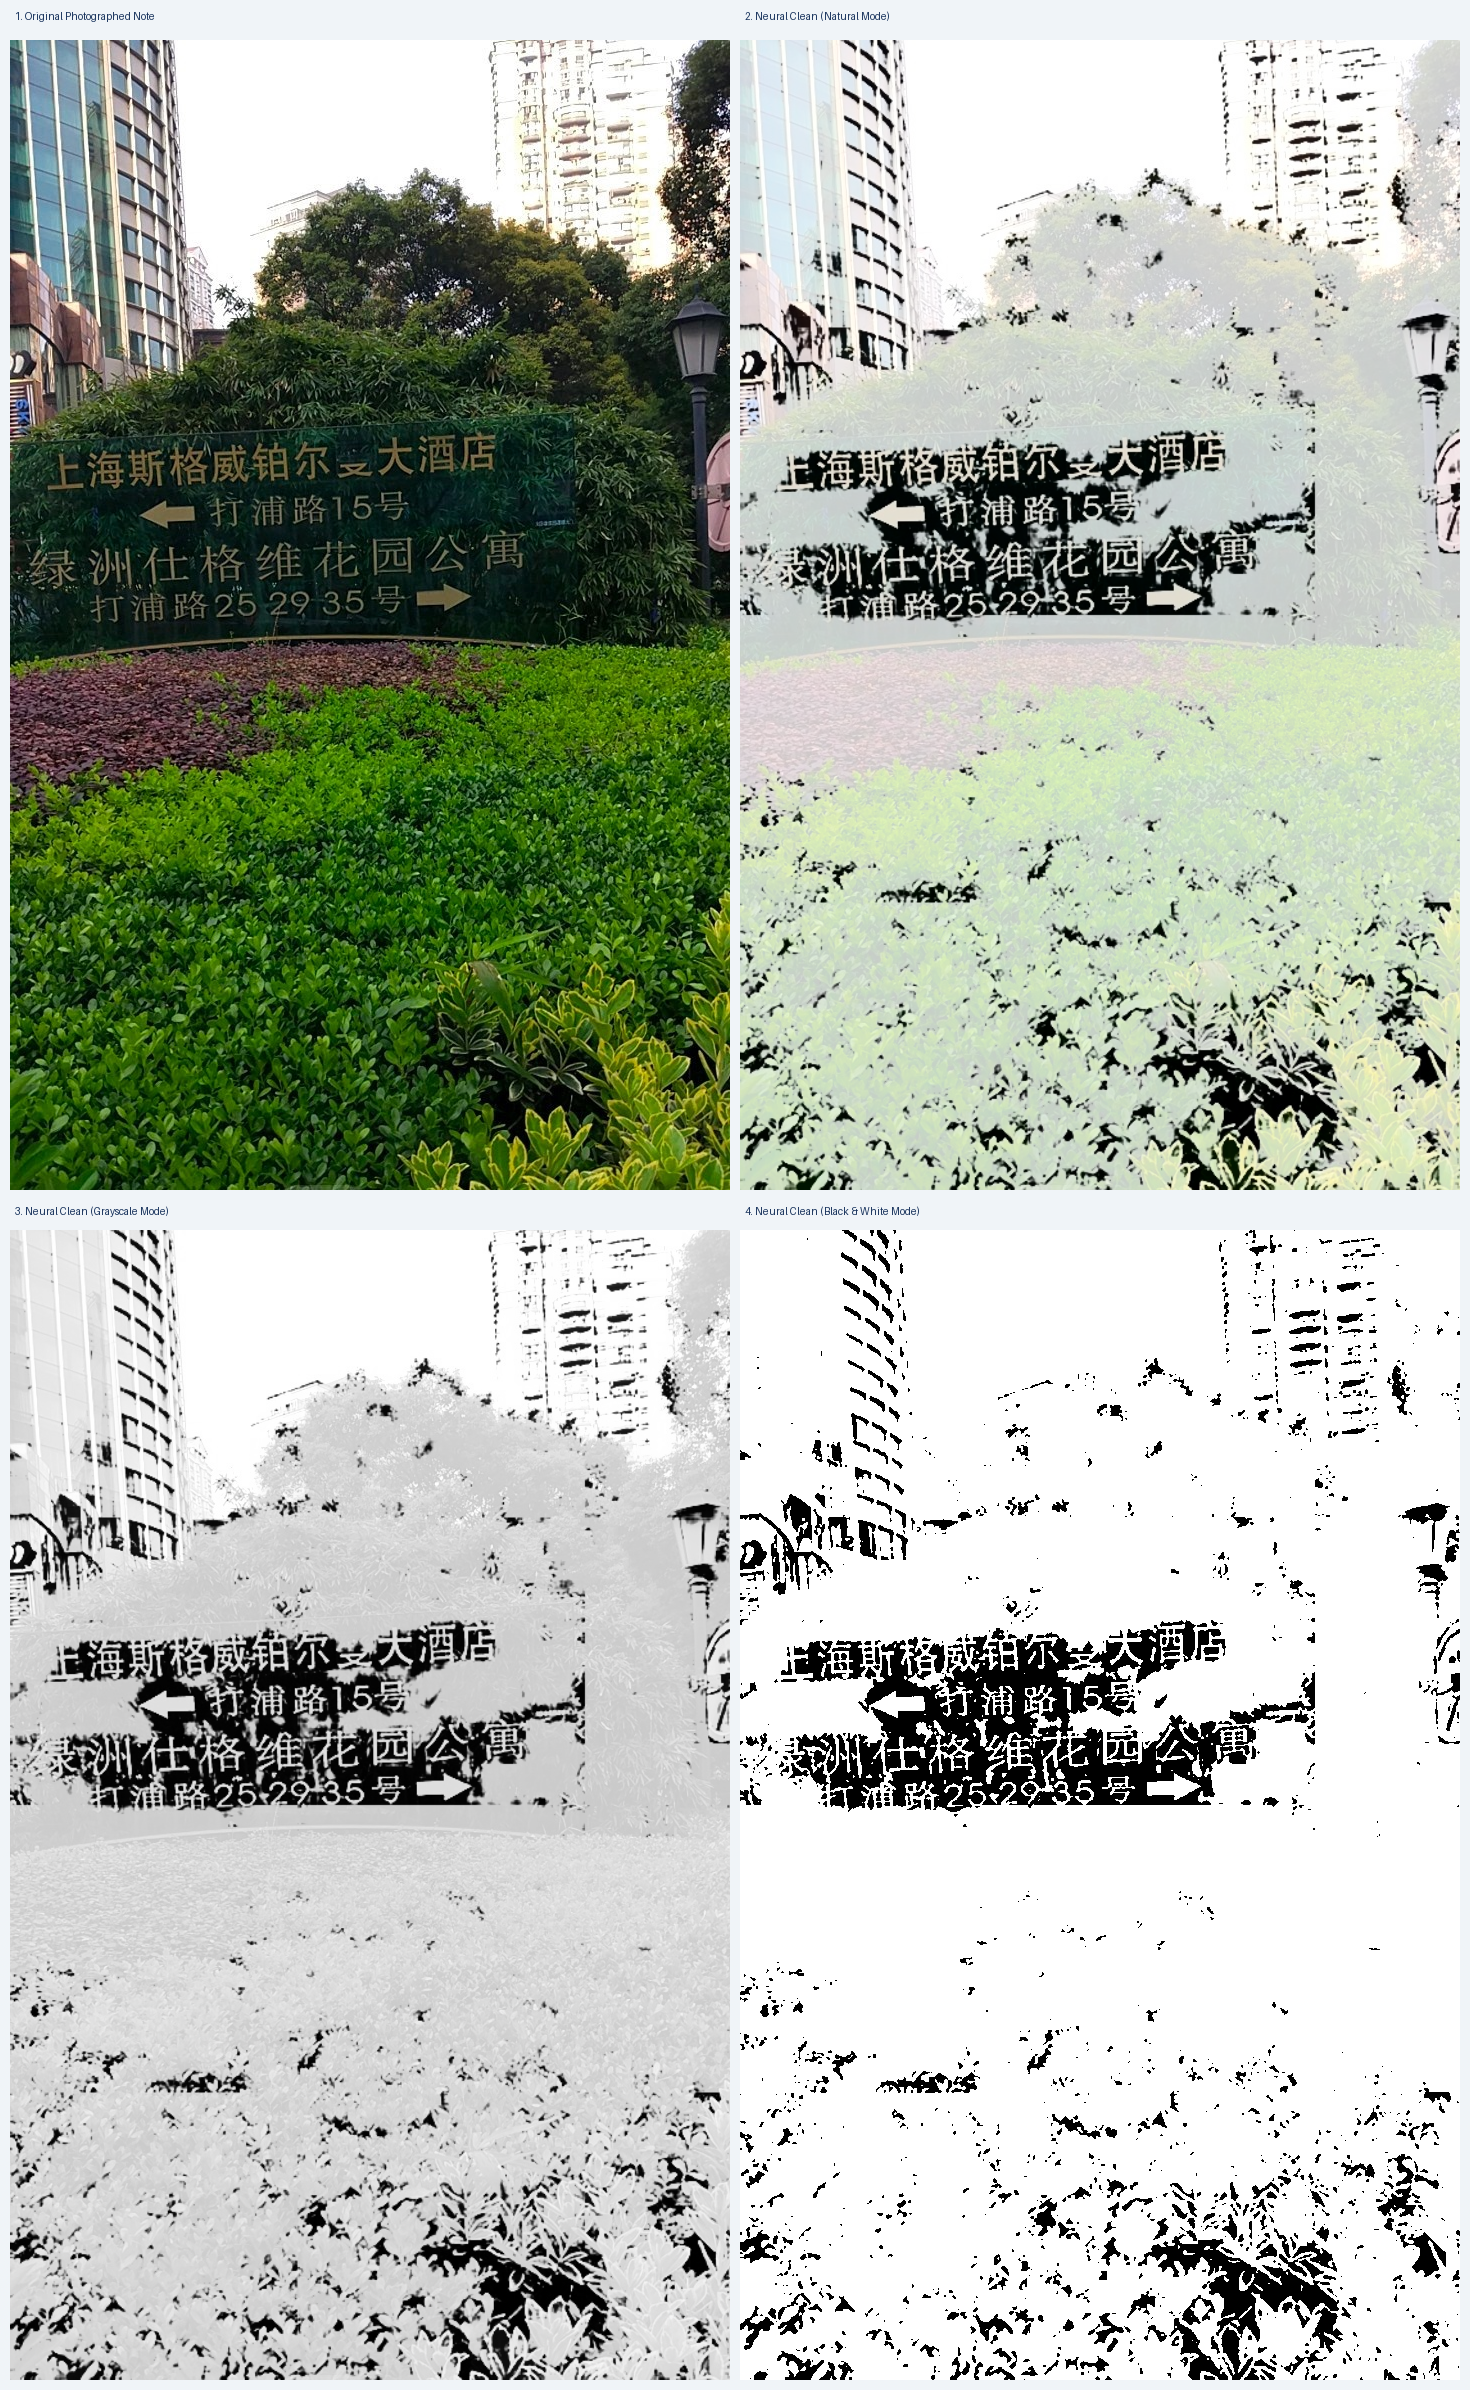
\includegraphics[width=0.96\linewidth]{demo_results/neural_clean_presentation_grid.png}
  \caption{Concept demonstration of the original note and Neural Clean rendering modes.}
  \label{fig:demo-clean}
\end{figure}

\begin{figure}[htbp]
  \centering
  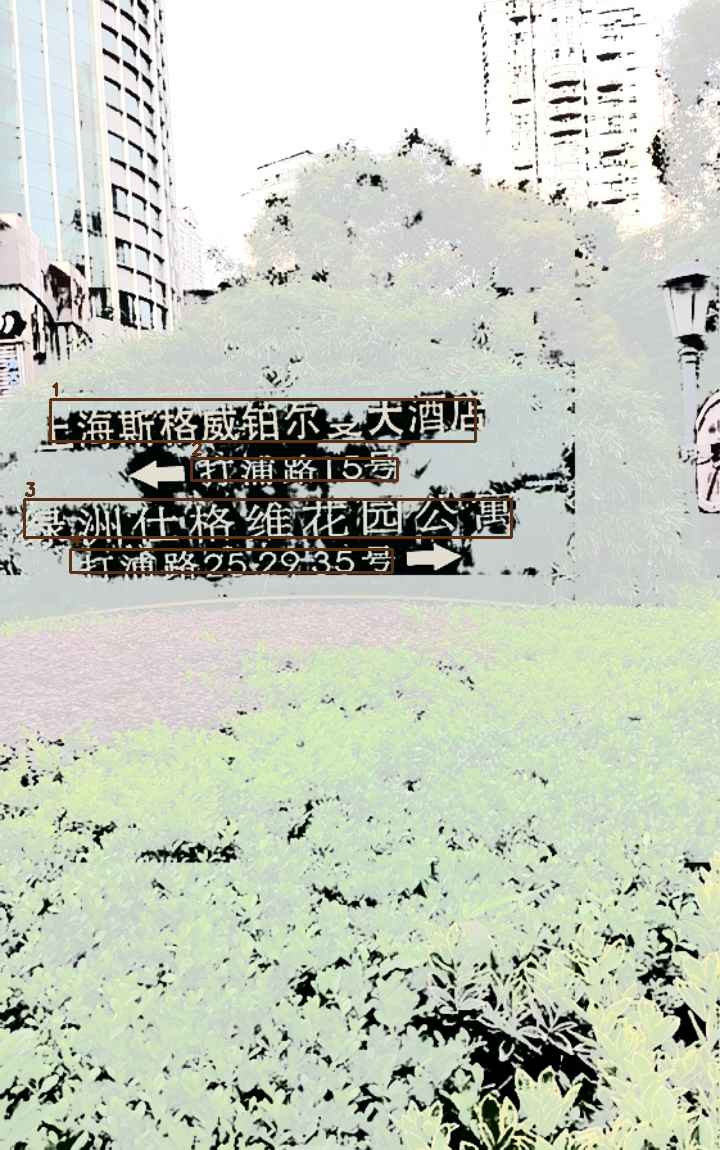
\includegraphics[width=0.96\linewidth]{demo_results/ocr_detection_boxes.png}
  \caption{PP-OCRv5 text-region detection result on the demo image.}
  \label{fig:demo-ocr}
\end{figure}

\subsection{Unit \& Formatter Tests}
Local JUnit tests verify horizontal whitespace collapse, paragraph retention, leading/trailing whitespace removal, Unicode safety, and sigmoid numerical stability.

\subsection{Instrumented End-to-End Tests}
Five instrumented tests pass on Android API 35/37 emulators:
\begin{enumerate}[leftmargin=*]
  \item Verifies that all bundled model assets exist and \texttt{INTERNET} permission is absent.
  \item Confirms that \textbf{Recognize text} remains disabled until an image is loaded.
  \item Validates text rendering, editing, scrolling, and character count updates in \texttt{OcrResultActivity}.
  \item Runs real PP-OCRv5 detection and recognition end-to-end offline on \texttt{ocr\_reference.png}.
  \item Runs real LiteRT \texttt{NeuralDocumentEnhancer} inference end-to-end offline.
\end{enumerate}

\section{Limitations \& Future Work}

\begin{itemize}[leftmargin=*]
  \item \textbf{Handwriting Complexity:} Highly cursive, overlapping, or blurred handwriting can reduce OCR accuracy.
  \item \textbf{Language Scope:} Optimised primarily for English text.
  \item \textbf{Hardware Acceleration:} Current inference runs on CPU threads (\texttt{XNNPACK}). Future releases can integrate NNAPI or GPU delegates for faster processing.
  \item \textbf{Evaluation Dataset:} Future benchmarks will evaluate Character Error Rate (CER) and Word Error Rate (WER) using the IAM Handwriting Database across disjoint writers.
\end{itemize}

\section{Conclusion}

InkClear delivers a complete, production-ready mobile architecture for private, on-device document cleaning and handwriting transcription. By integrating pretrained LiteRT and ONNX models directly inside the application package and enforcing strict permission boundaries, InkClear proves that modern neural AI tools can provide high utility while guaranteeing absolute user privacy.

\end{document}